%!TEX root = ../../thesis.tex

\section{Research Questions}
\label{sec:research-questions}

In the last section, we discuss a few central research questions in this field, which still remain as open questions and yet to be answered in the future.

\subsection{How to Measure Progress?}
The first question is: \ti{How can we measure the progress of this field?} The evaluation metrics are certainly clear indicators of measuring progress on our reading comprehension benchmarks. Does this indicate that we make real progress on reading comprehension in general? How can we tell if some progress on one benchmark can generalize to others? How about if model $A$ works better than model $B$ on one dataset, while model $B$ works better on the other dataset? How to tell how far these computer systems are sill from genuine human-level reading comprehension?

On the one hand, we think that taking human's standardized tests could be a good strategy for evaluating the performance of machine reading comprehension systems. These questions are usually carefully curated and designed to test human's reading comprehension abilities at different levels. To get computer systems aligned with human measurements is a proper way in building natural language understanding systems.
% {\red{TODO: Not always correct --- some questions are easy for humans to answer but difficult for machines}}.

On the other hand, we believe that it would be desirable to integrate many reading comprehension datasets as a testing suite for evaluation in the future, instead of only testing on one single dataset. This will help us better distinguish what are genuine progress for reading comprehension and what might be just overfitting to one specific dataset.

More importantly, we need to understand our existing datasets better: characterizing their quality and what skills are required to answer the questions. This will be a crucial step for building more challenging datasets and analyzing the behavior of our models. Besides our work on analyzing the \sys{CNN/Daily Mail} examples in \newcite{chen2016thorough}, \newcite{sugawara2017evaluation} attempted to separate reading comprehension skills into two disjoint sets: \ti{prerequisite skills} and \ti{readability}.  Prerequisite skills measure different types of reasoning and knowledge required to answer the question and 13 skills are defined: object tracking, mathematical reasoning, coreference resolution, logical reasoning, analogy, causal relation, spatiotemporal relation, ellipsis, bridging, elaboration, meta-knowledge, schematic clause relation and punctuation. Readability measures the “text ease of processing”, and a wide range of linguistic features/human readability measurements are used. The authors concluded that these two sets are weakly correlated and it is possible to design difficult questions from the contexts that are easy to read. These studies suggest that we could construct datasets and develop models based on these properties separately.

In addition, \newcite{sugawara2018what} designed a few simple filtering heuristics and divided the examples from many existing datasets into a hard subset and an easy subset, based on 1) whether the question can be answered using only the first few words; 2) whether the answer is contained in the most similar sentence in the passage. They observed that the baseline performances for the hard subsets remarkably degrade compared to those of the entire datasets. Moreover, \newcite{kaushik2018how} analyzed the performance of existing models using passage-only or question-only information, and found that these models sometimes can work surprisingly well and hence there exists annotation artifacts in some of the existing datasets.

In conclusion, we believe that if we want to make steady progress on reading comprehension in the future, we will have to answer these basic questions about the difficulty of examples first. Understanding what is required for the datasets, what our current systems can do and can't do will help us identify the challenges we are facing and measure the progress.

\subsection{Representations vs. Architecture: Which is More Important?}
\label{sec:rep-vs-arch}

\begin{figure}[!t]
    \center
    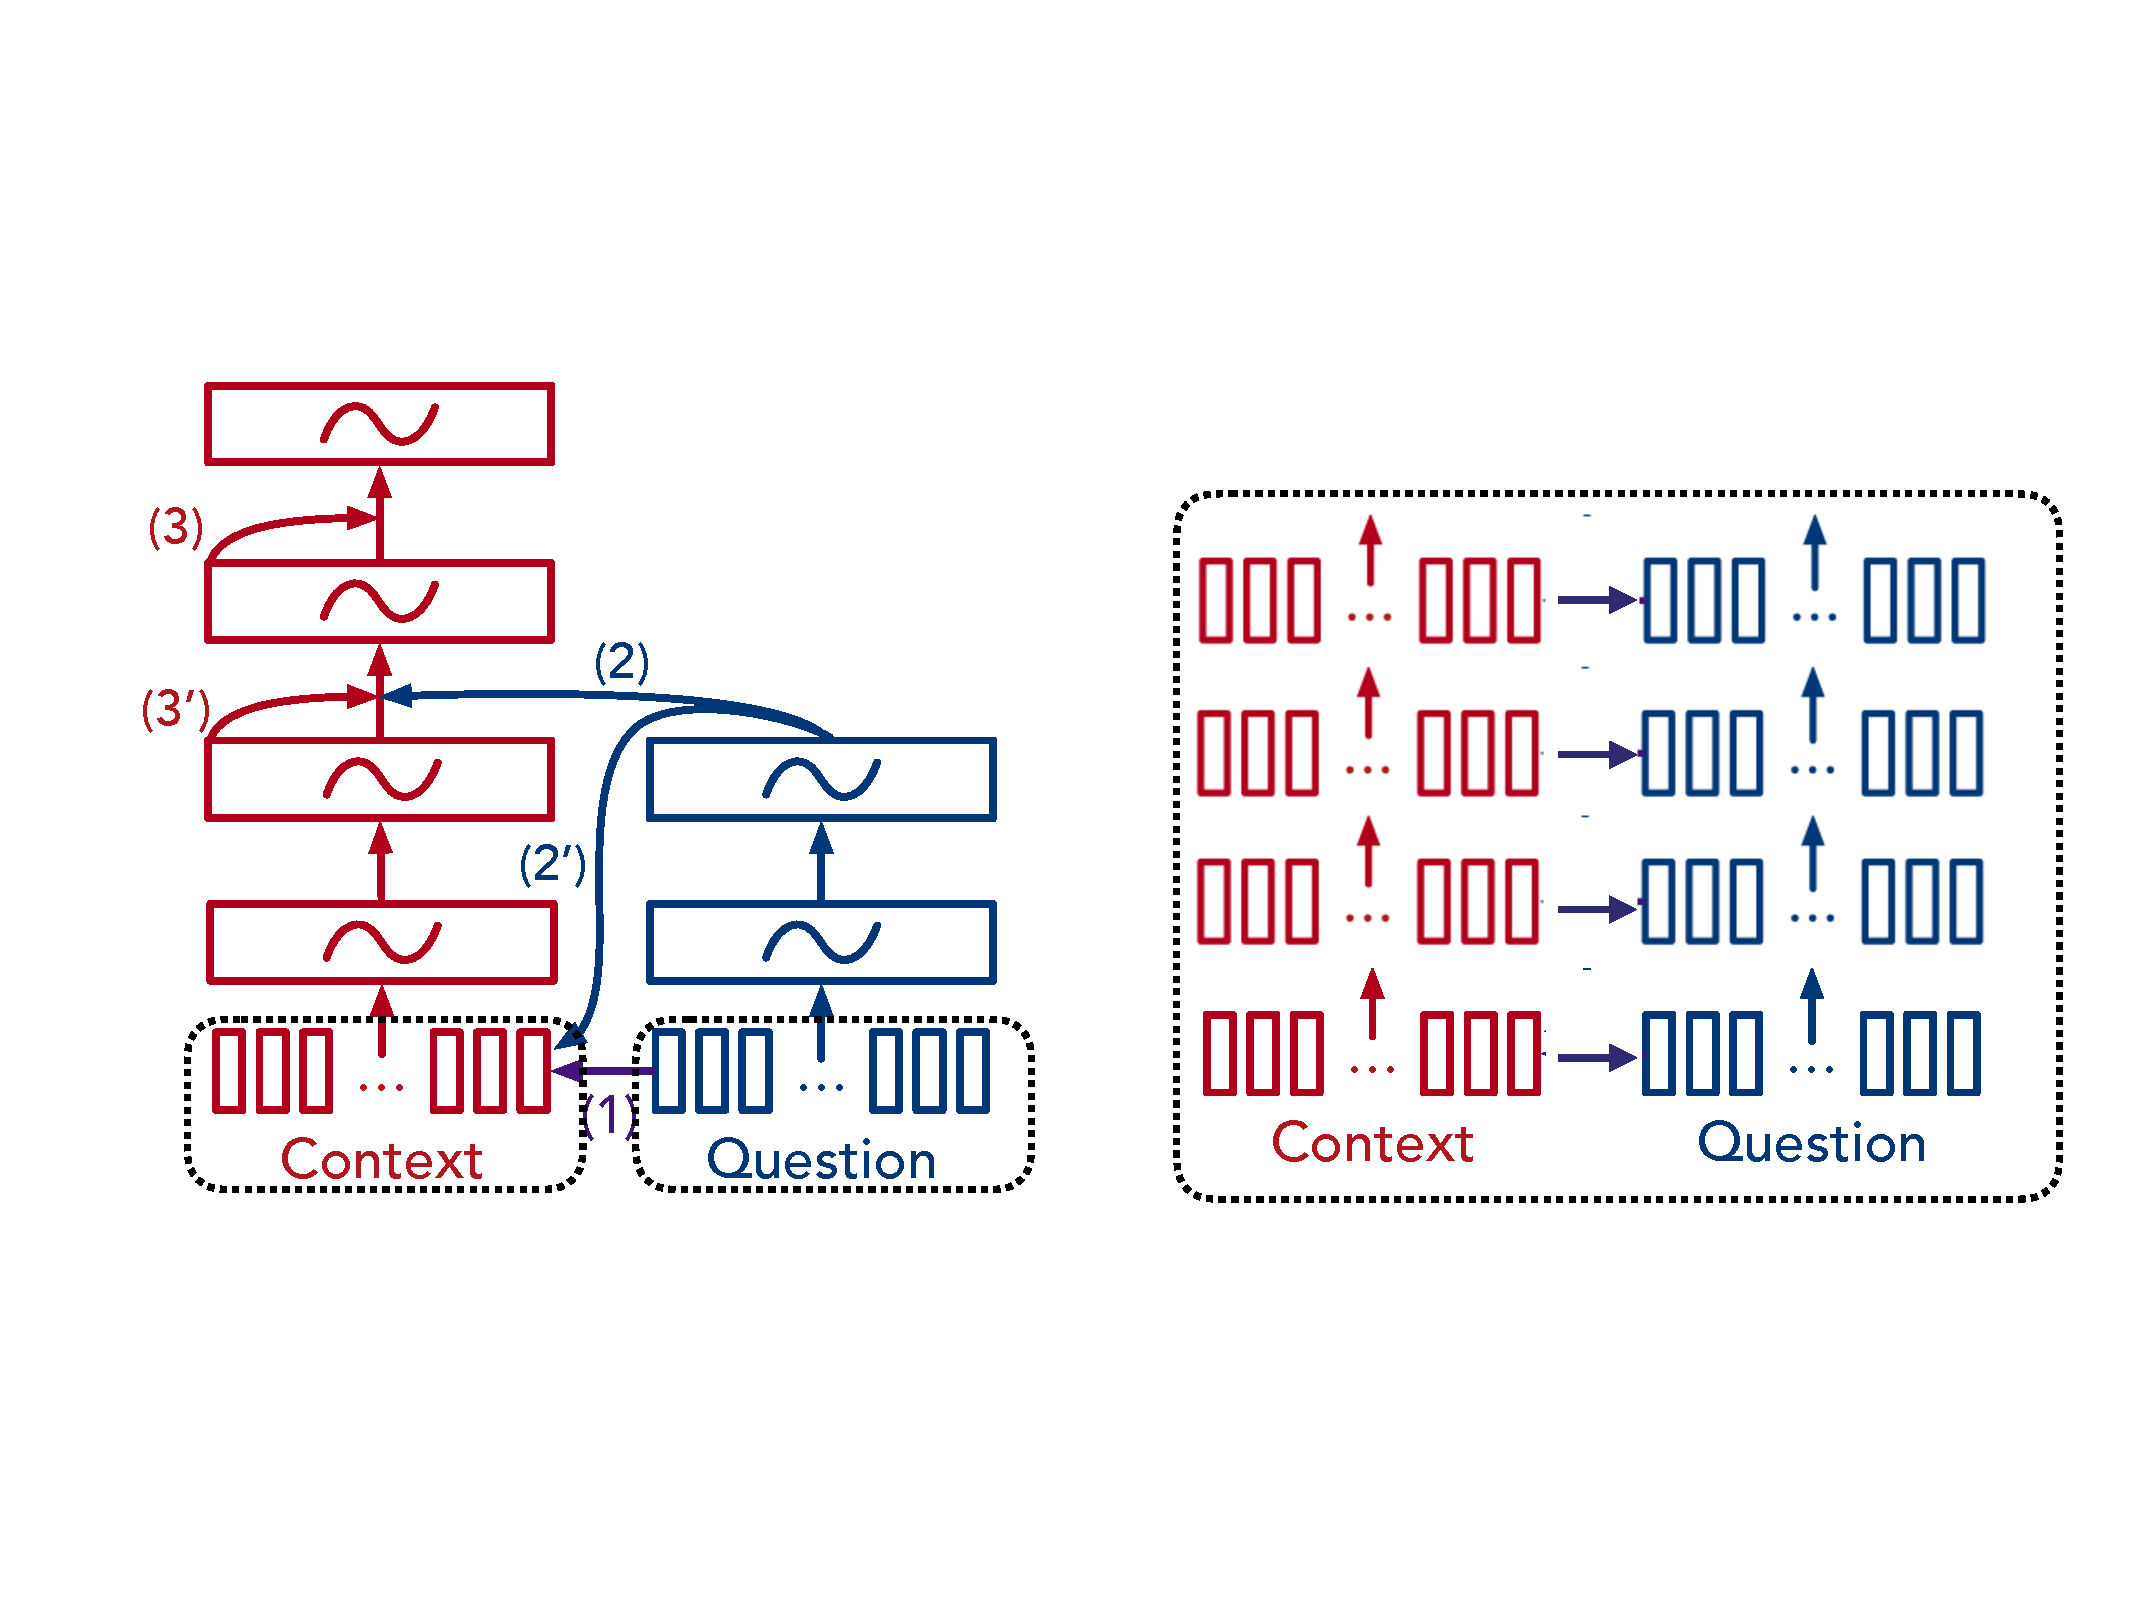
\includegraphics[scale=0.45]{img/rep_vs_arch.pdf}
    \longcaption{A comparison of a complex architecture vs. a simple architecture with pre-training}{\label{fig:rep-vs-arch}A comparison of a complex architecture (left) vs. a simple architecture with pre-training (right). The parameters in the dashed box can be pre-trained from unlabeled text, while all the remaining parameters are initialized randomly and learned from the reading comprehension datasets.}
\end{figure}

The second important question is to understand the role of representations vs. architectures to the performance of reading comprehension models. Since \sys{SQuAD} was created, there has been a recent trend of increasing the complexity of neural architectures. In particular, more and more complex attention mechanisms have been proposed to capture the similarity between the passage and the question (Section~\ref{sec:attention-mechanisms}). However, recent works~\cite{radford2018improving,devlin2018bert} proposed that if we can pretrain a deep language model on large text corpora, a simple model which takes the concatenation of the question and the passage without modeling any direct interactions between the two can work extremely well on reading comprehension datasets such as \sys{SQuAD} and \sys{RACE} (see Table~\ref{tab:squad-results} and Table~\ref{tab:recent-datasets}).

As illustrated in Figure~\ref{fig:rep-vs-arch}, the first class of models (left) only builds on top of word embeddings (each word type has a vector representation) pre-trained from unlabeled text, while all the remaining parameters (including all the weights to compute various attention functions) need to be learned from the limited training data. The second class of models (right) makes the model architecture very simple and it only models the question and passage as a single sequence. The whole model is pre-trained and all the parameters are kept. Only a few new parameters are added (e.g., the parameters for predicting the start and end positions for \sys{SQuAD}) and the other parameters will be fine-tuned on the training set of the reading comprehension tasks.

We think these two classes of models indicate two extremes. On the one hand, it certainly demonstrates the incredible power of unsupervised representations. As we have a powerful language model pre-trained from huge amount of text, the model already encodes a great deal of properties about language while a simple model which concatenates the passage and the question is sufficient to learn the dependency between the two. On the other hand, when only word embeddings are given, it seems that modeling the interactions between the passage and the question carefully (or giving the model more prior knowledge)  helps. In the future, we suspect that we will need to combine the two and a model like \sys{BERT} is too coarse to handle the examples which require complex reasoning.


\subsection{How Many Training Examples Are Needed?}
The third question is \ti{how many training examples are actually needed?} We have discussed many times that the success of neural reading comprehension is driven by large-scale supervised datasets. All the datasets that we have been actively working on contain at least 50,000 examples. Can we always embrace data abundance and further improve the performance of our systems? Is it possible to train a neural reading comprehension model with only hundreds of annotated examples today?

We think there isn't a clear answer yet. On the one hand, there is clear evidence that having more data helps. \newcite{bajgar2016embracing} demonstrated that inflating the cloze-style training data constructed from books available through project Gutenberg can provide a boost of 7.4\%--14.8\% on the \sys{Children Book Test (CBT)} dataset~\cite{hill2016goldilocks} using the same model. We discussed before that using data augmentation techniques~\cite{yu2018qanet} or augmentating the training data with \sys{TriviaQA} can help improve the performance on \sys{SQuAD} (\# training examples = 87,599).

On the other hand, pre-trained (language) models~\cite{radford2018improving,devlin2018bert} can help us reduce the dependence on large-scale datasets. In these models, most of the parameters are already pretrained on abundant unlabeled data and will be only fine-tuned during training.

In the future, we should encourage more research on unsupervised learning and transfer learning. Leveraging unlabeled data (e.g., text) or other cheap resources or supervision (e.g., datasets like \sys{CNN/Daily Mail}) will relieve us from collecting expensive annotated data. We also should seek better and cheaper ways of collecting supervised datasets.
%
% \red{Chris: I think the main substantive thing missing here is a discussion of more difficult types of questions that probe deeper levels of Reading Comprehension. That is a middle school reading comprehension exercise normally is not so much about answering factoid style questions that but showing that you understood the reasoning and implications of the text and what the author is trying to convey. Often this is done with how/why questions: In the story, why is Cynthia upset with her mother? How does John attempt to make up for his original mistake? How does the author indicate that Benjamin is scared to be left alone? But there are other aspects of deeper comprehension too. We can argue about how successful they have been, but I think very clearly the goal of the AI2 Aristo work has been to try to have comprehension tests where you actually have to understand the underlying science of what is being discussed, rather than just answering from text matching. It would be good to have a paragraph or two on issues like this --- assessing deeper reading comprehension than question text matching.}
